\subsection{Komponente der Datenverarbeitung}
Gem�� der Abbildung \ref{wissenserwerbskomponente} stellt die Datenverarbeitungskomponente ein Bindeglied zwischen der Wissensbasis (hier Git-Repository) und den Wissenserfassungsverfahren (z.B. Wissenstr�gerschnittstelle) dar. Auf Implementierung bezogen handelt es sich um ein Programm, das f�r eine kleine Aufgabe zust�ndig ist. Martin Flowler bezeichnet das als Mircoservice\footnote{https://www.martinfowler.com/articles/microservices.html}. Im Fall von \textit{PaaSfinder} wird dieser Microservice als \glqq{}Worker\grqq{} bezeichnet. Schematisch wird der Worker in Abbildung \ref{fig:worker} dargestellt.
\begin{figure}[H] 
	\centering
	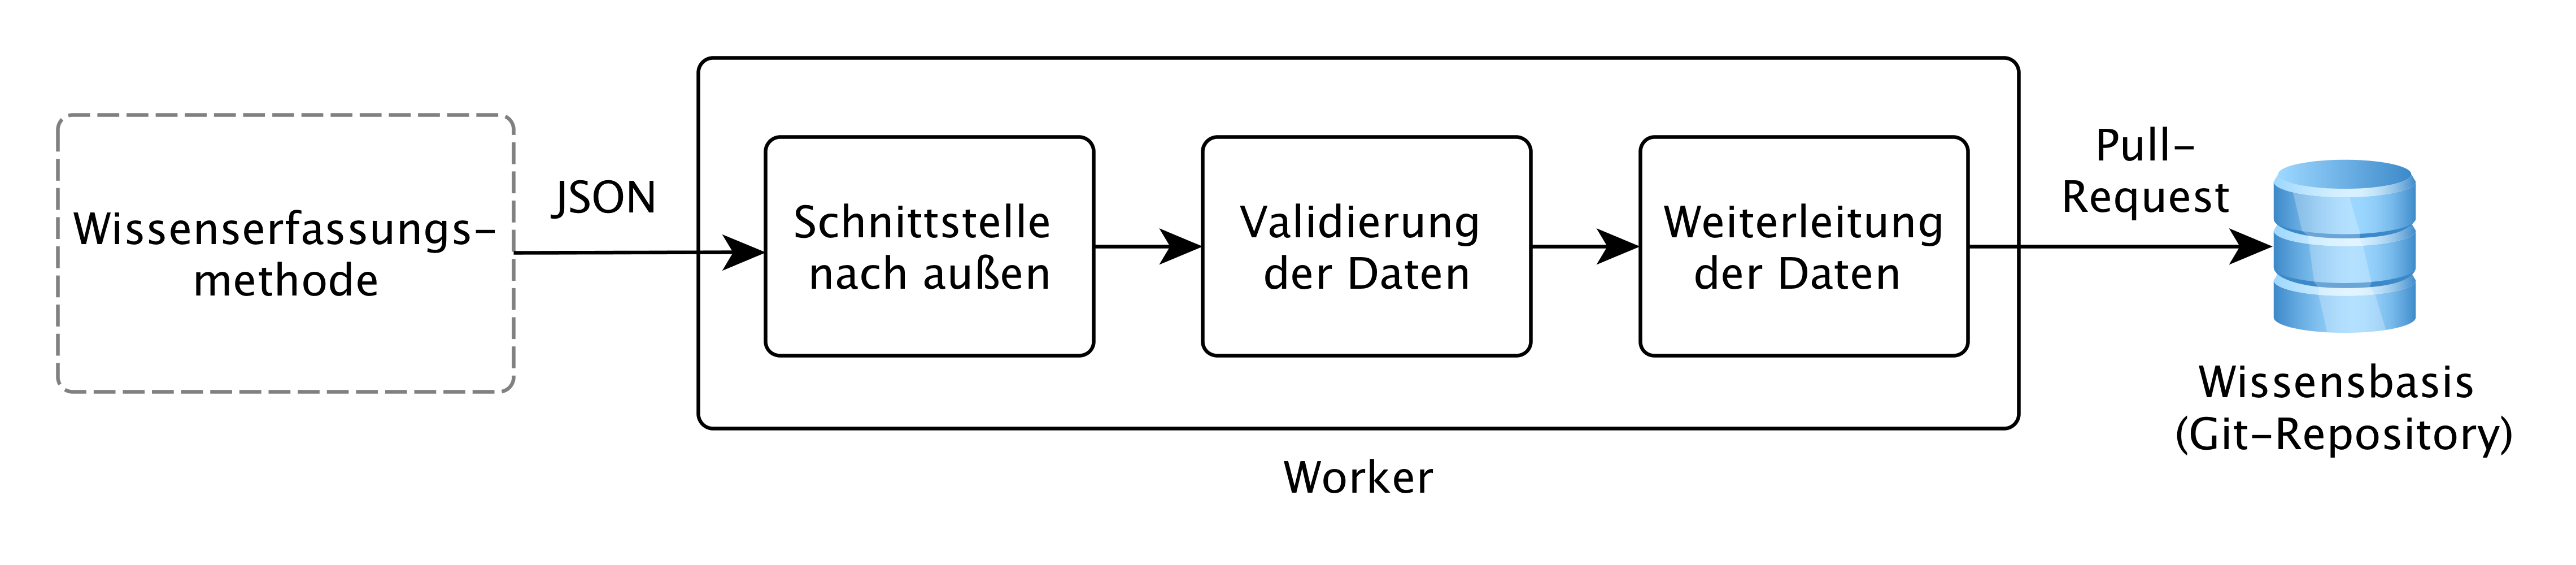
\includegraphics[width=0.99\textwidth]{images/worker.png}
	\caption{Der Aufgabenbereich vom Worker}
	\label{fig:worker}
\end{figure}
Als erstes werden die Daten als ein JSON entgegengenommen. Im weiteren Schritt werden die Daten nach bestimmten Kriterien (z.B. der Name soll nicht null sein) gepr�ft und gegebenenfalls abgelehnt. Auch die Einschr�nkung, dass nur JSON Objekte akzeptiert werden, geh�rt zur Validierung. Anschlie�end werden die Daten bereitgestellt und als Pull-Request an das Repository geschickt.\\
Der Worker wird als \ac{REST}-API umgesetzt. \textit{Hier die Beschreibung von REST...} 